\chapter{平台实际效果}
平台 UI 界面主要包含了用户信息管理与交互式神经元编辑两部分界面,使用了 Ant Design\upcite{antdesign} 作为设计规范和组件设计语言,three.js\upcite{threejs} 作为 3D 引擎实现交互式实时 3D 神经元编辑。本章主要展示了前端界面,并分析了平台实际性能。

\section{前端界面展示}
图 \ref{login} 展示了用户登录界面,图 \ref{register} 展示了用户注册界面,图中的“Hatu”是平台名称。

\begin{figure}[!ht]
\begin{minipage}[t]{0.5\linewidth} 
    \centering  
    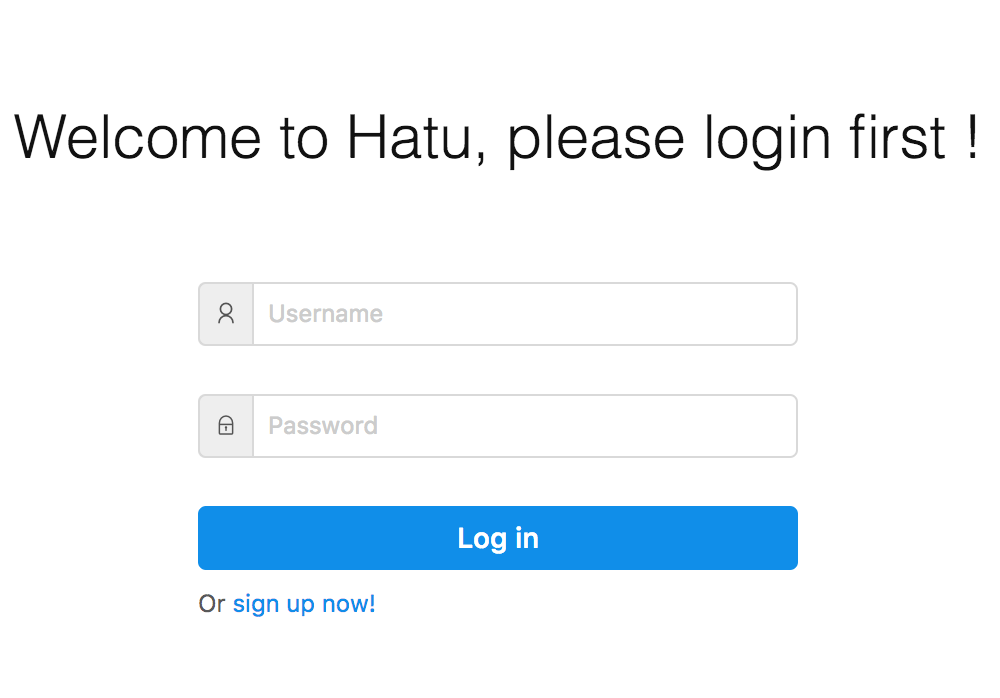
\includegraphics[width=7cm]{images/login}  
    \caption{用户登录界面}
    \label{login}  
    \end{minipage}  
    \begin{minipage}[t]{0.5\linewidth}
    \centering  
    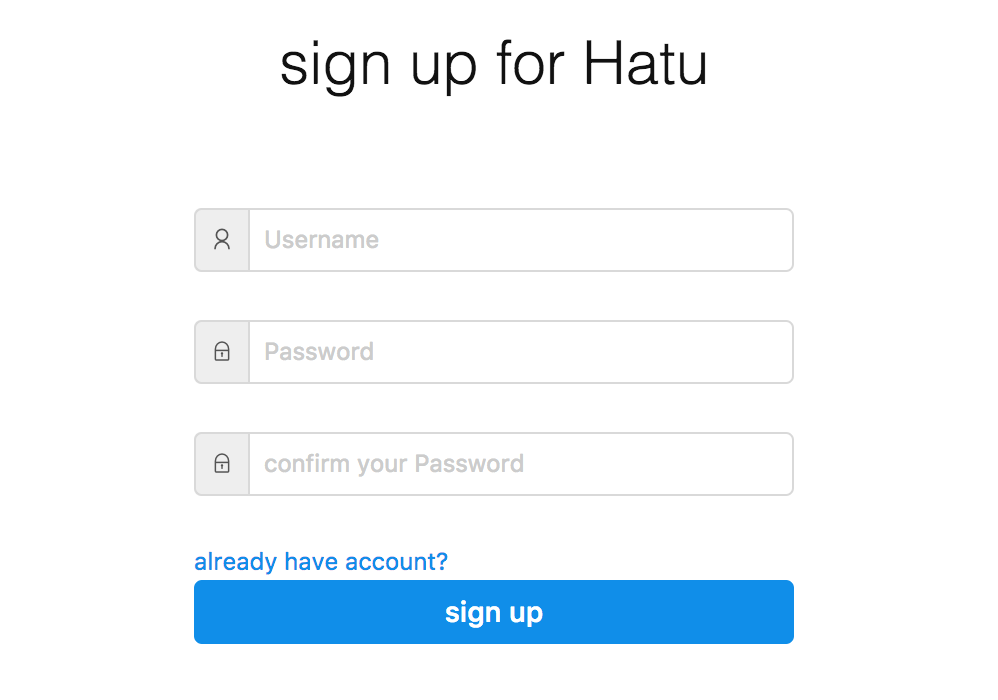
\includegraphics[width=7cm]{images/register}  
    \caption{用户注册界面}  
    \label{register}  
    \end{minipage}  
\end{figure}

\begin{figure}[!ht]
\begin{minipage}[t]{0.5\linewidth}
    \centering  
    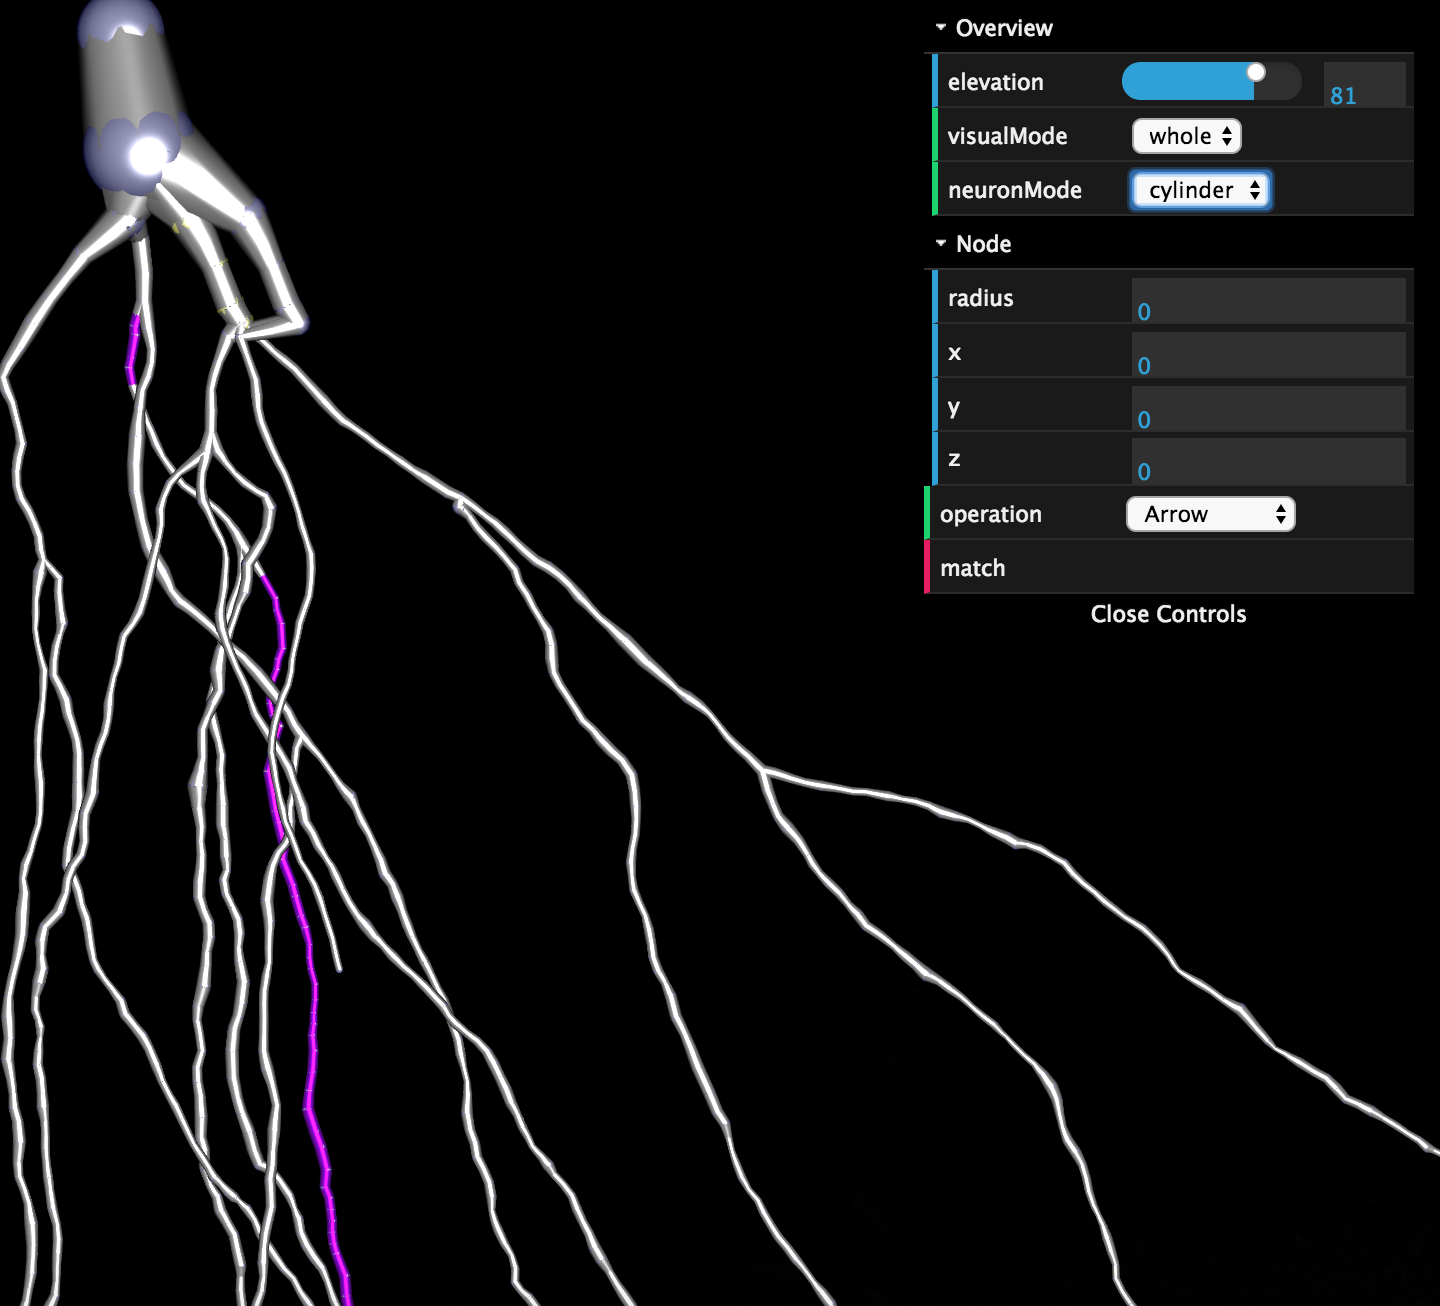
\includegraphics[width=7cm]{images/cylinder}  
    \caption{3D 柱状模式下交互式编辑界面}
    \label{cylinder}  
    \end{minipage}  
    \begin{minipage}[t]{0.5\linewidth} 
    \centering  
    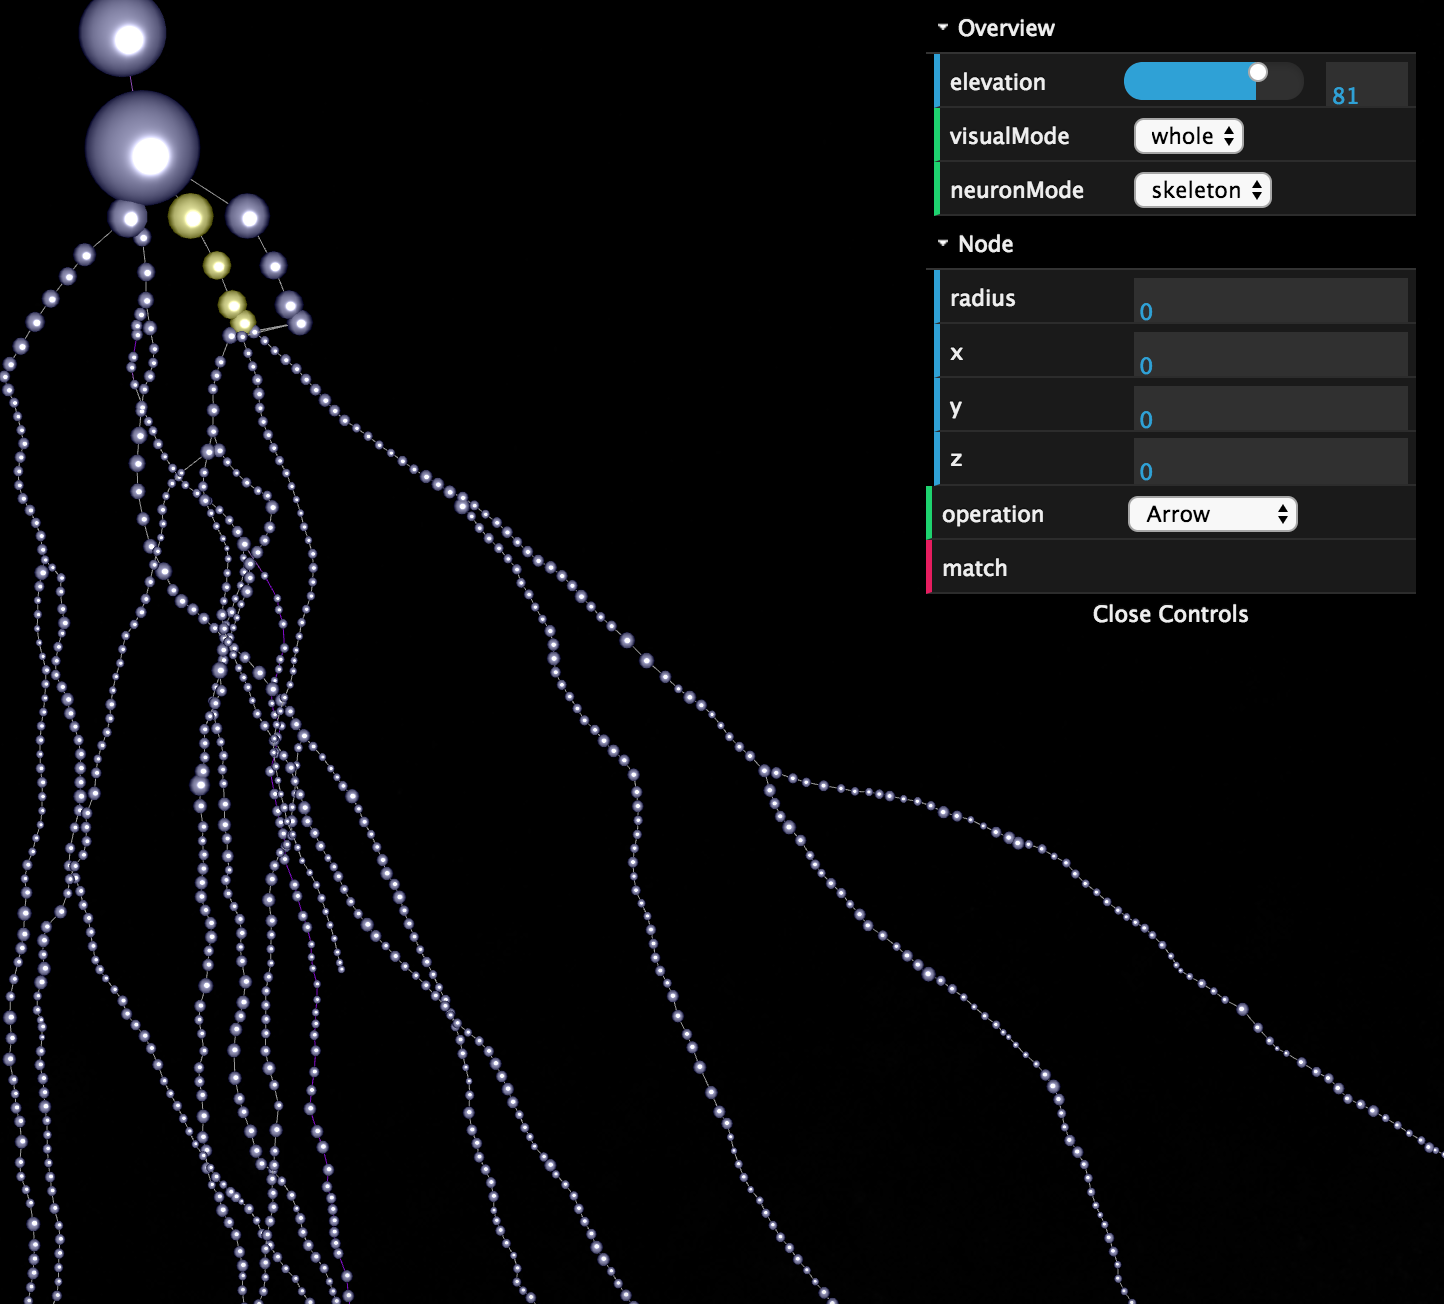
\includegraphics[width=7cm]{images/skeleton}  
    \caption{3D 骨架模式下交互式编辑界面}  
    \label{skeleton}  
\end{minipage} 
\begin{minipage}[t]{0.5\linewidth}
    \centering  
    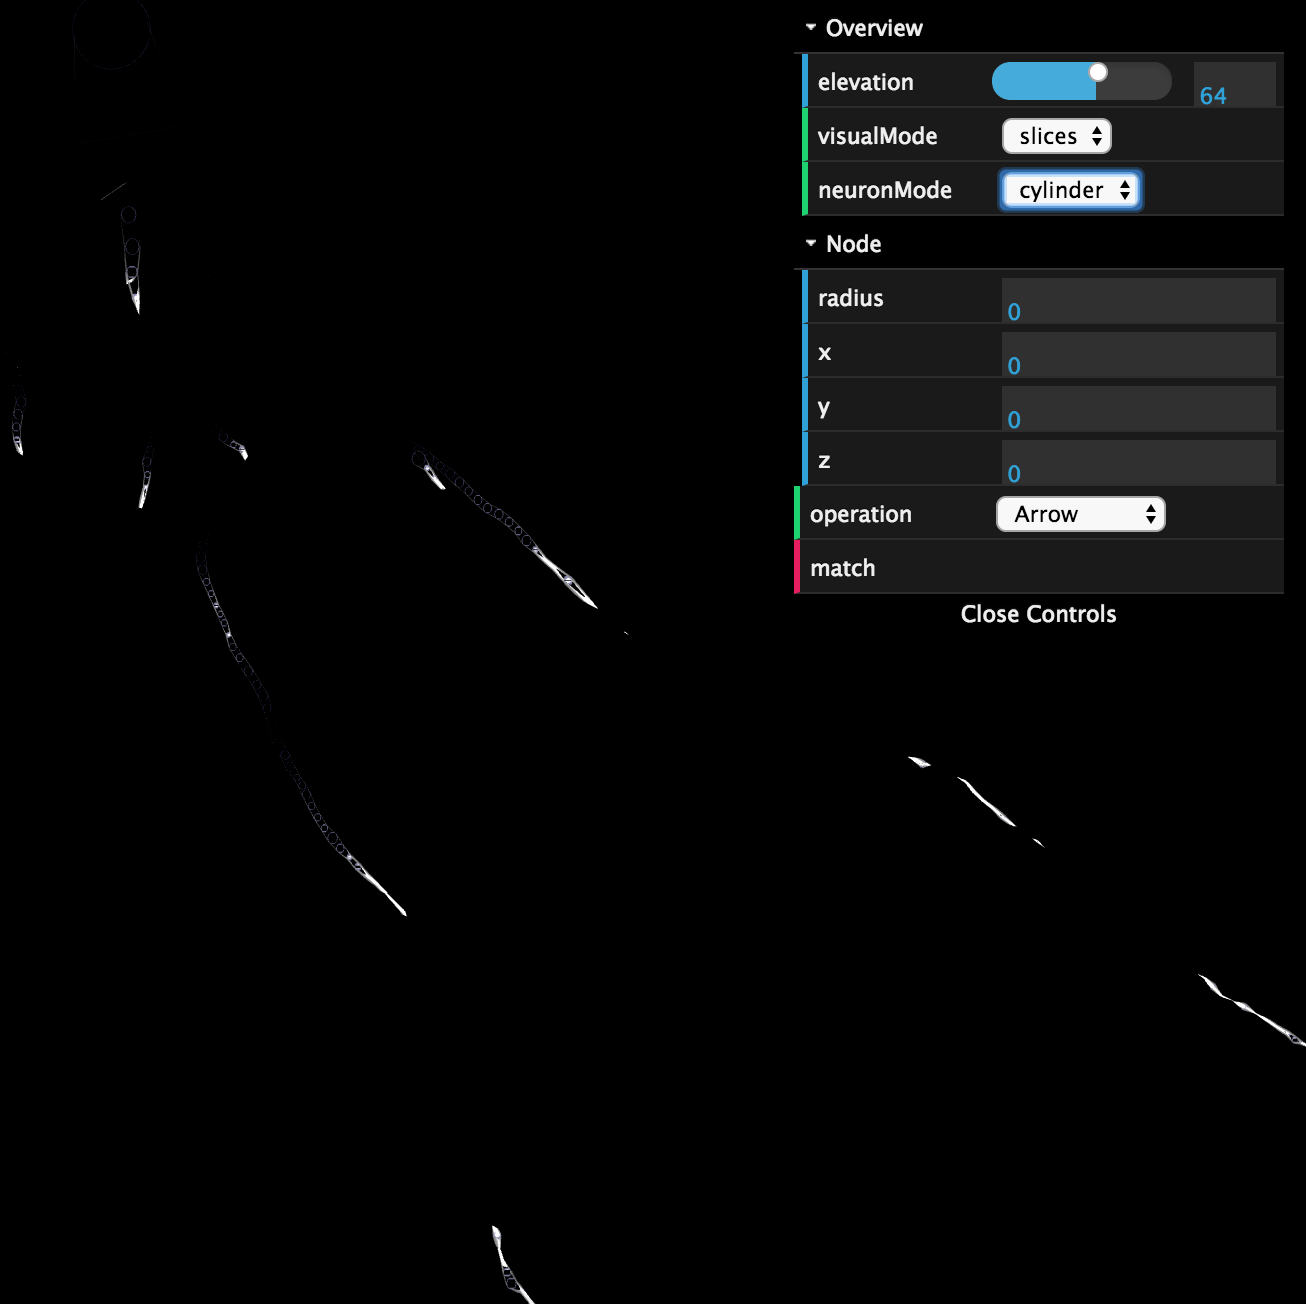
\includegraphics[width=7cm]{images/slice}  
    \caption{2D 切片模式下交互式编辑界面}
    \label{slice}  
\end{minipage}   
\end{figure}

\begin{figure}[!ht]
\begin{minipage}[t]{0.19\linewidth}
    \centering  
    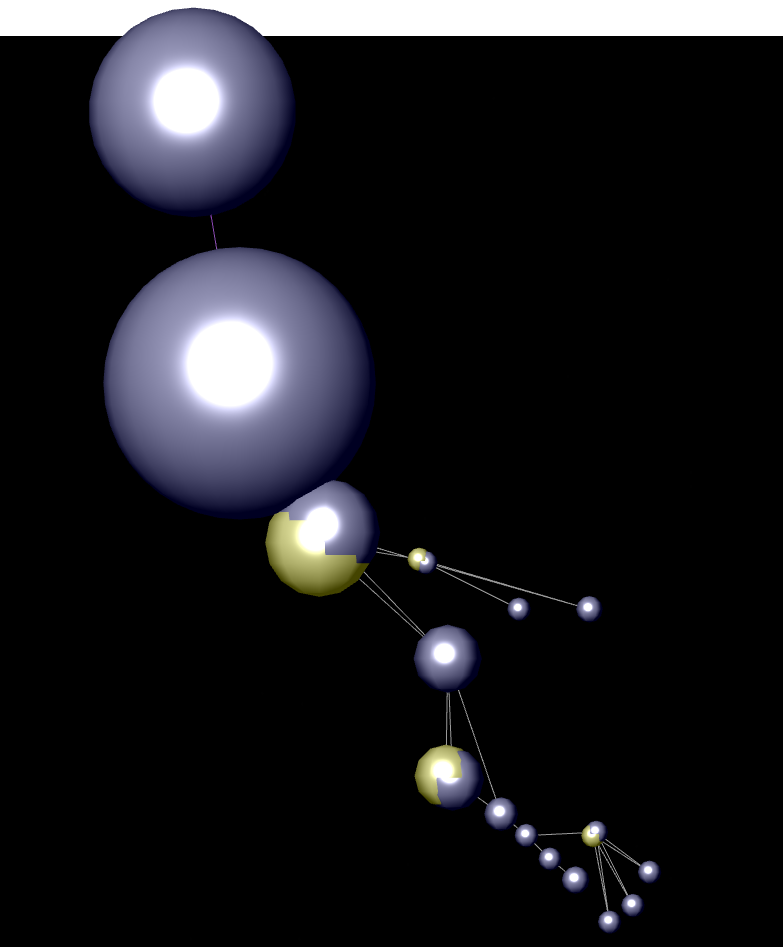
\includegraphics[width=2.8cm]{images/a0}   
\end{minipage}  
\begin{minipage}[t]{0.19\linewidth} 
    \centering  
    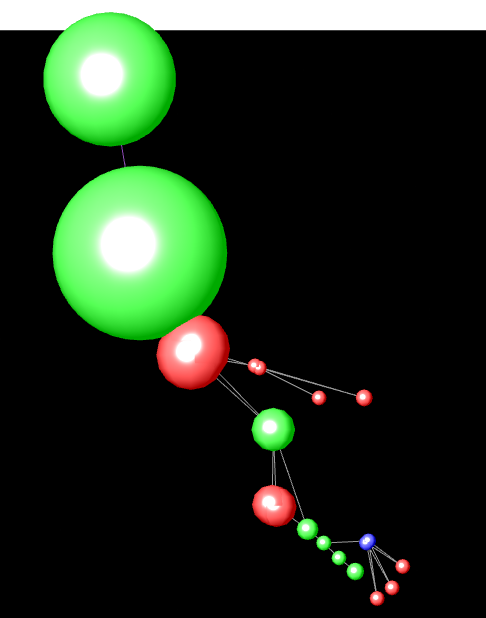
\includegraphics[width=2.8cm]{images/a1}  
\end{minipage} 
\begin{minipage}[t]{0.19\linewidth}
    \centering  
    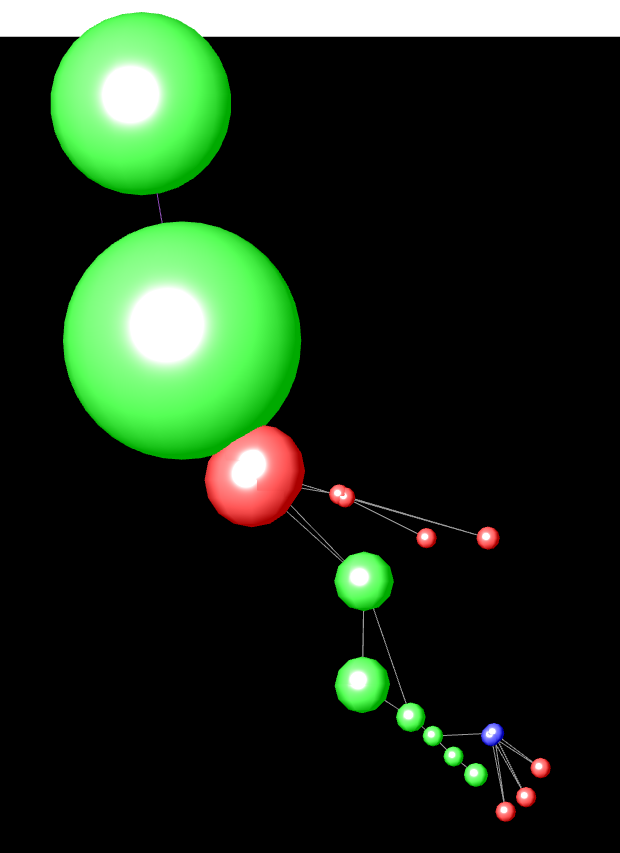
\includegraphics[width=2.8cm]{images/a2}    
\end{minipage}   
\begin{minipage}[t]{0.19\linewidth}
    \centering  
    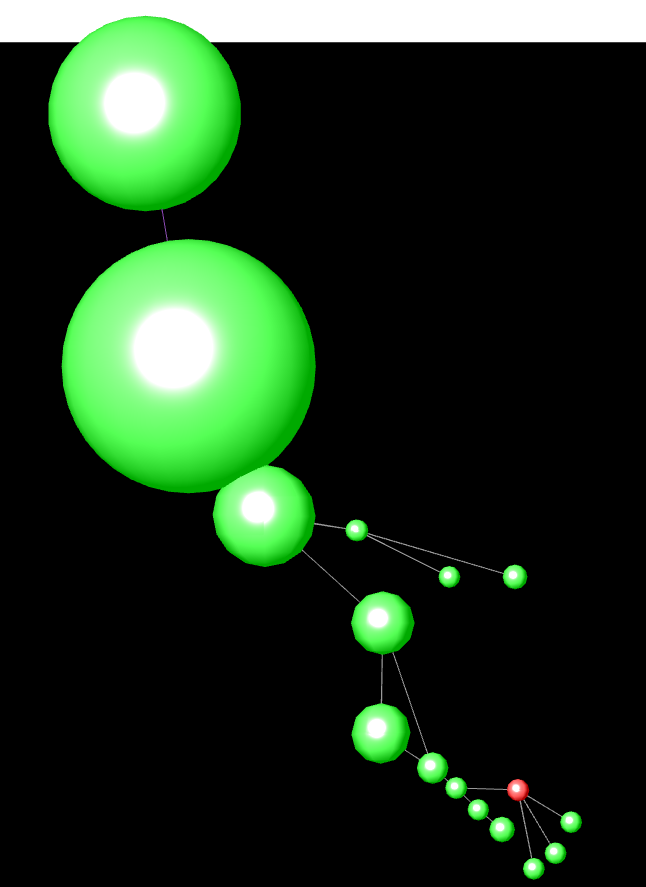
\includegraphics[width=2.8cm]{images/a3}   
\end{minipage}   
\begin{minipage}[t]{0.19\linewidth}
    \centering  
    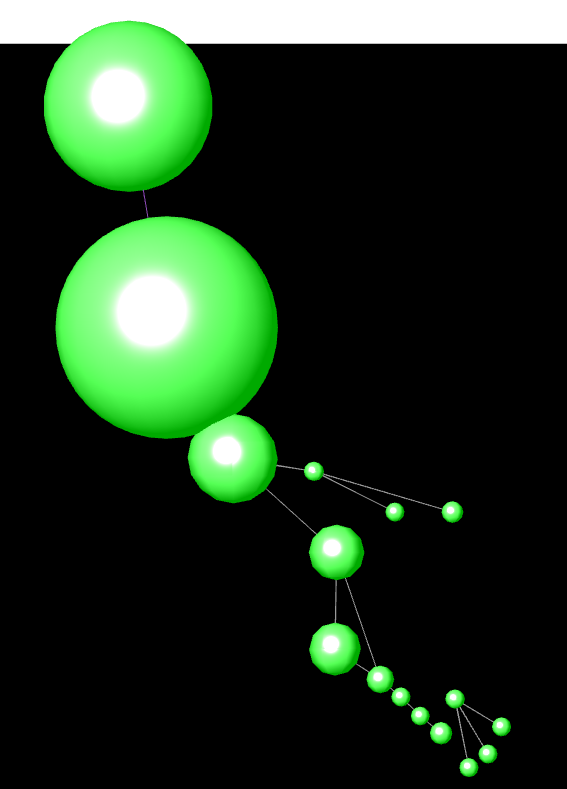
\includegraphics[width=2.8cm]{images/a4}   
\end{minipage} 
\caption{多用户协同编辑时结果合并的操作序列}
\label{merge}     
\end{figure}

图 \ref{cylinder} 展示了 3D 柱状模式下交互式编辑界面,图 \ref{skeleton} 展示了 3D 骨架模式下交互式编辑界面,图 \ref{slice} 展示了 2D 切片模式下交互式编辑界面。不同交互模式的适用场景不同。3D 模式适用于概览神经元整体结构,但是不适合精心调整,尤其不适合调整深度信息。2D 界面适合精细调整,可以和原始切片图像信息进行对比,保证调整的精确度,但是只能看到一个切片内的信息,难以查看神经元结构整体。神经科学家在使用时应根据具体的使用场景选取不同的模式。

图 \ref{cylinder} 与图 \ref{skeleton} 展示 3D 模式下用不同颜色的球标明了团队中其他人员的修改,当前编辑人员可以决定保存团队中其他人员的修改或者进一步进行修改,系统会自动根据两者的修改内容进行半自动合并,图 \ref{merge} 展示了多用户协同编辑时结果合并的操作序列,这部分算法由同组海杰文完成,本文不详细论述。在编辑完成之后可以选择将编辑成果分享给其他神经科学家,使得团队协作变得更加简洁。

\section{前端请求实际性能}
\subsection{静态文件请求}
经过 webpack 打包过后只有两个 js 文件与一个 css 文件。两个 js 文件中一个是前端程序员编写的代码另一个是依赖的第三方代码。图 \ref{file-nocache} 示了静态资源文件的大小与第一次获取的时间。由于可视化任务较为复杂,即使在压缩过后仍有 2MB 左右的大小,在第一次未缓存的状况下有 4s 的加载时间,用户能明显地感受到加载时间。图 \ref{file-cache} 展示了缓存后的加载时间,此时只需要一百毫秒的时间即可完成加载,也就是说用户在后续的访问中不会感受到延迟。 

\begin{figure}[!ht]
\centering
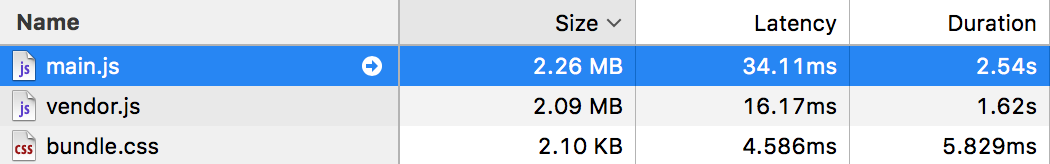
\includegraphics[width=148mm]{images/file-nocache}
\caption{静态资源文件大小与未缓存时所需的加载时间}
\label{file-nocache}
\end{figure}

\begin{figure}[!ht]
\centering
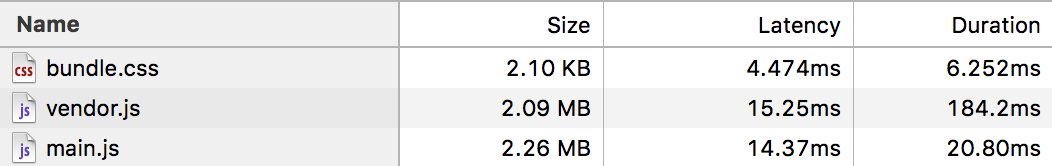
\includegraphics[width=148mm]{images/file-cache}
\caption{静态资源文件大小与缓存后所需的加载时间}
\label{file-cache}
\end{figure}

\subsection{登录与注册请求}
图 \ref{login-res} 展示了用户登录请求响应时间,图 \ref{signup-res} 展示了用户注册响应时间。从图中可以看出登录请求用时 24.40 ms,注册请求用时 183.37ms,属于用户可以接受的范围内。注册请求较登录请求响应时间更长是由于注册新用户是需要初始化神经信息数据库,这需要消耗一定的时间。

\begin{figure}[!ht]
\centering
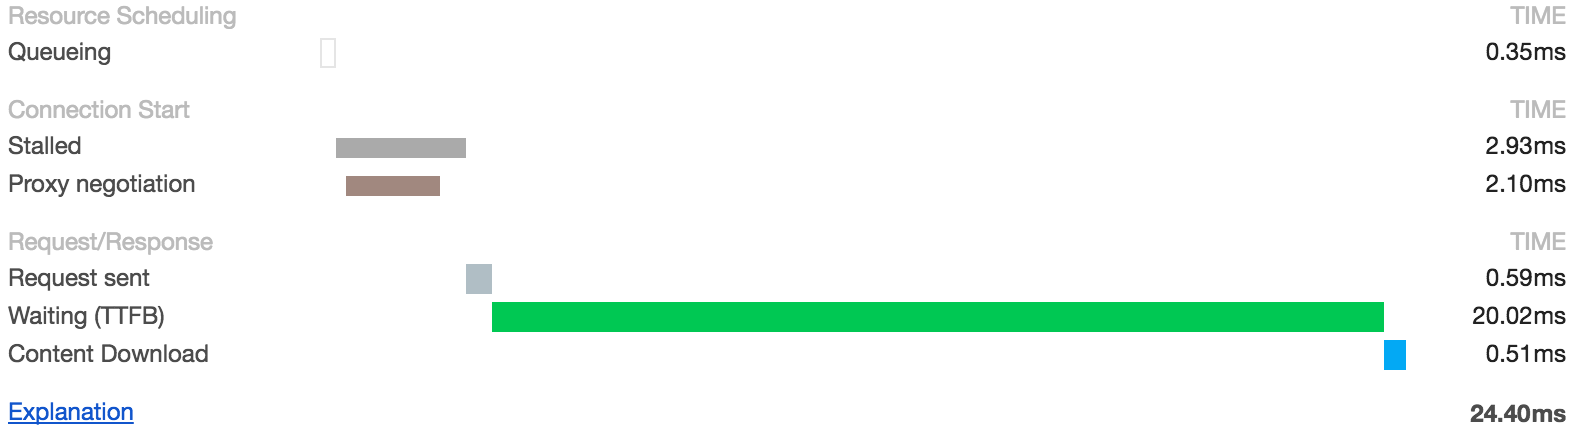
\includegraphics[width=128mm]{images/login-res}
\caption{用户登录请求响应时间}
\label{login-res}
\end{figure}

\begin{figure}[!ht]
\centering
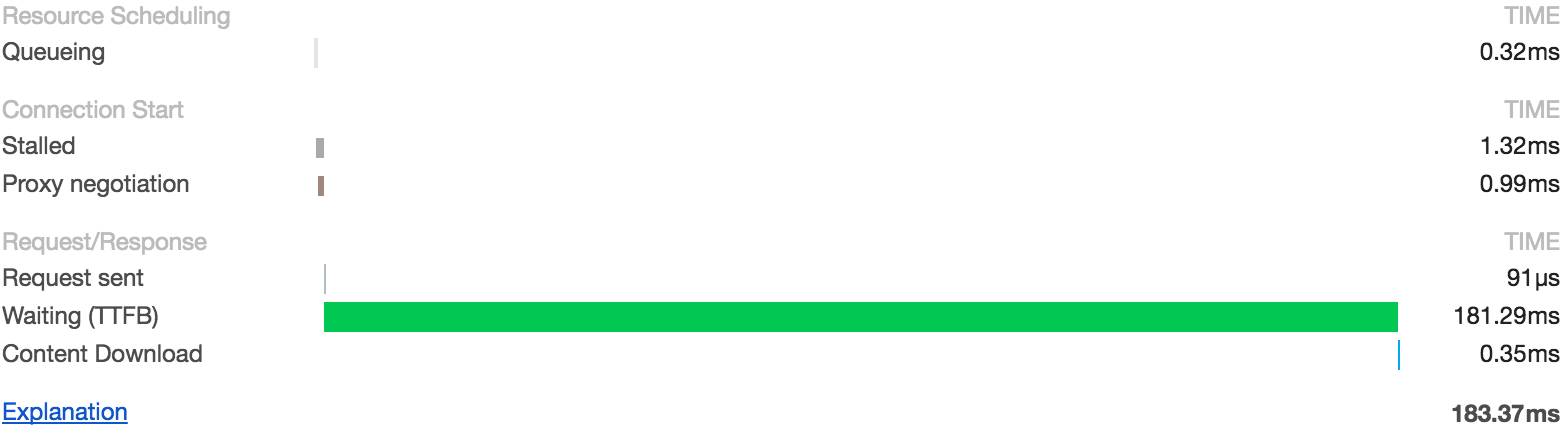
\includegraphics[width=128mm]{images/signup-res}
\caption{用户注册请求响应时间}
\label{signup-res}
\end{figure}

\subsection{动态请求}
图 \ref{dy-res} 展示了动态请求的大小,数据和\ref{chap3}中测试数据一致,最长响应时间在 100ms 左右,用户不会感受到明显的卡顿。值得注意的是两个 slice15 请求和两个 slice15\_L11.swc 请求。两次请求的响应时间一个从 89.37ms 下降到 37.95ms,另一个从 109.0ms 下降到 13.50ms 再一次说明了使用缓存对性能的巨大提升。

\begin{figure}[!ht]
\centering
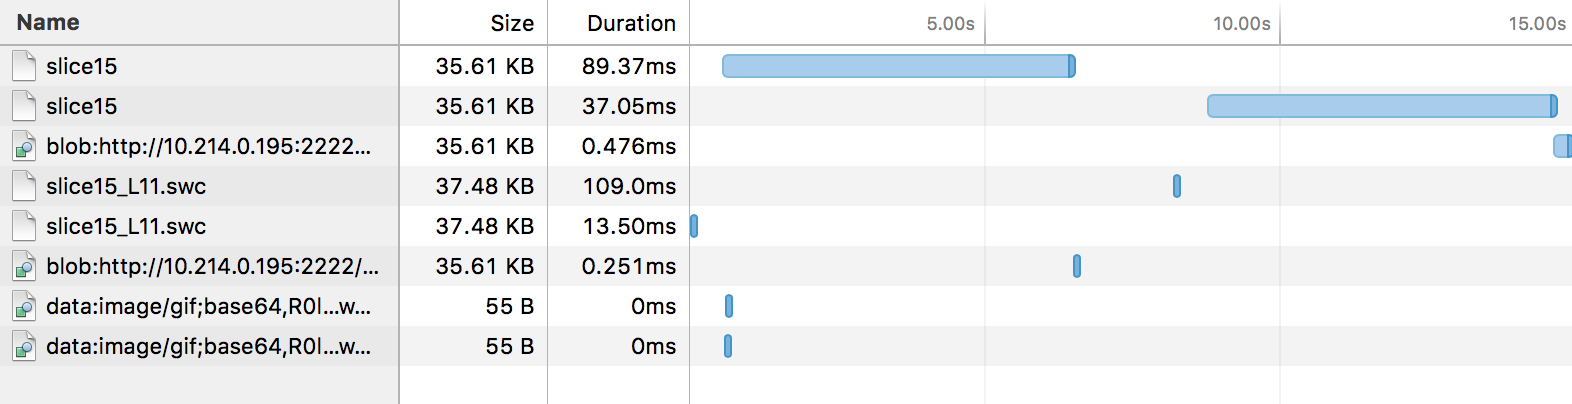
\includegraphics[width=148mm]{images/dy-res}
\caption{动态请求大小与请求响应时间}
\label{dy-res}
\end{figure}

\section{本章小结}
本章展示了用户信息管理与交互式神经元编辑两部分前端界面,并详细分析了静态文件请求,登录与注册请求与动态请求三种前端请求,与\ref{chap3}中压力测试的结果进行验证。绝大多数的请求均可在毫秒级别响应,保证了前端可视化与编辑操作的流畅。目前存在的问题是两个 js 文件过大,用户在第一次访问时能感受到明显的加载时间。需要进一步研究相关技术,压缩 js 文件的大小。